\subsection{Story: Admins can log into the website and run a session with a quiz}
\subsubsection{Analysis - breakdown of tasks}
After doing some spike work in the previous iteration, this task can now be approached and broken into several sub tasks:
\begin{itemize}
	\item Set up config for Pusher
	\item Add event for broadcasting
	\item Write a command to trigger this event
	\item Add a button to quizzes to trigger this event
	\item Display the response on the front end using the JavaScript which listens for Pusher events
	\item Add a session key box to front page
	\item Add session\_id to admin users and allow them to change it
	\item When admin clicks run, this session\_id can be entered into the key box to join a channel with the name of the id
	\item The user will be presented with the initial quiz page which will be filled with the name and description of the quiz by default
	\item The admin will see the same page but with an "admin panel"
	\item This admin panel has a next and previous button for questions
	\item When these buttons are pressed, the question is sent to pusher
	\item These question are rendered as a form on the user end and admin end
	\item The user can submit the form
\end{itemize}
\subsubsection{Design}
Mockups of the student end of the system figures \ref{fig:quiz-desktop} and \ref{fig:quiz-mobile}. Use case of the frontend system figure \ref{fig:iter-4-use-case}.

\begin{figure}
	\caption{Design for a quiz on a desktop}
	\centerline{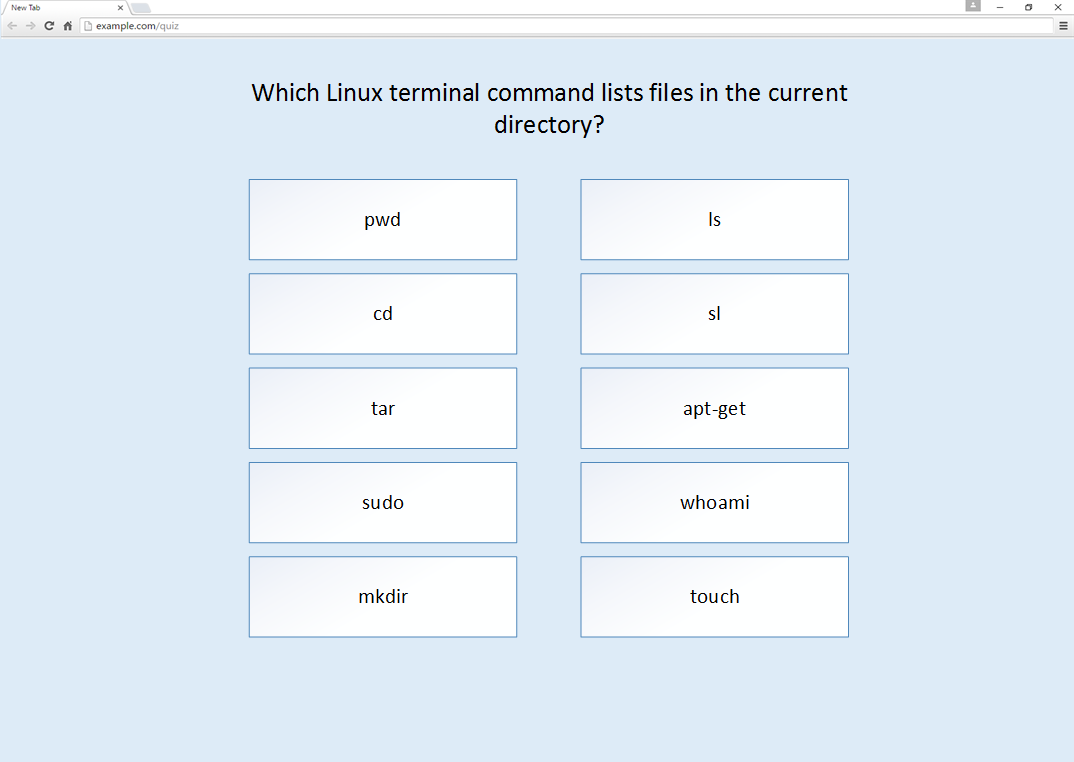
\includegraphics[width=\textwidth]{Chapter2/Iter-4/Quiz-Web-Design-Cropped}}
	\label{fig:quiz-desktop}
\end{figure}
\vspace{1cm}
\begin{figure}
	\caption{Design for a quiz on a mobile device}
	\centerline{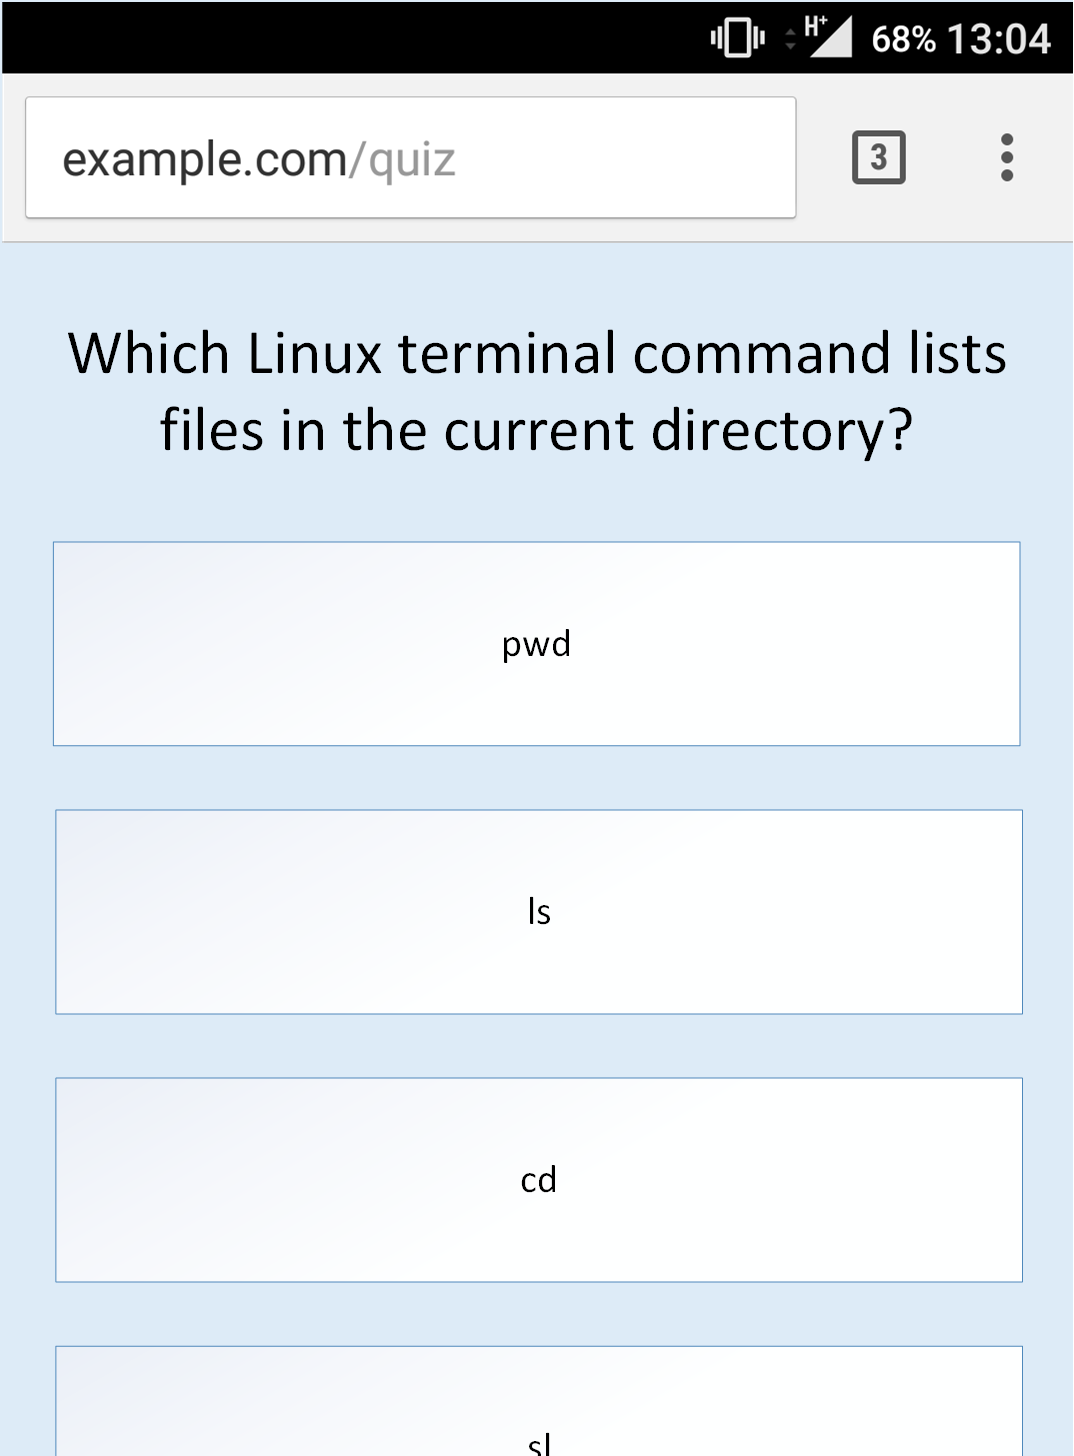
\includegraphics[scale=0.25]{Chapter2/Iter-4/Quiz-Mobile-Cropped}}
	\label{fig:quiz-mobile}
\end{figure}
	
\begin{figure}
	\caption{Use case diagram with the quiz control functionality. Omitted backend extends and includes to make more readable. See previous iterations for more complete backend use case.}
	\centerline{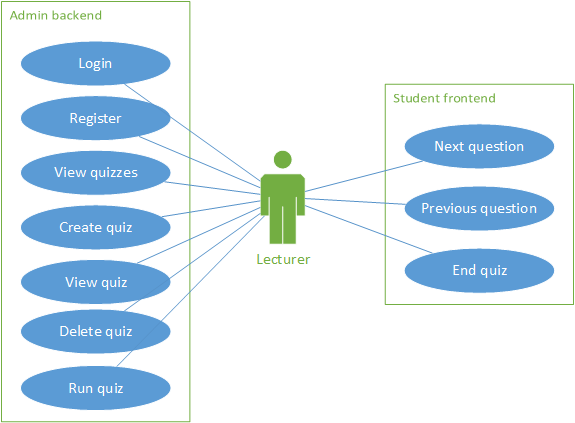
\includegraphics{Chapter2/Iter-4/iter-4-use-case}}
	\label{fig:iter-4-use-case}
\end{figure}

When the event is triggered, quiz data will be sent to Pusher, which will then send back this data to the channel specified. The session page will be listening on that channel, and this data can be appended to the page using JavaScript.

\subsubsection{Implementation}
Work began by configuring Pusher, creating an event and writing some basic JavaScript to append the data to the front page. Work was also done on the admin panel, making it only visible to logged in users (the lecturer running the quiz), and adding the functionality for previous and next question buttons. These are buttons that send Ajax requests to quiz controller actions which then trigger the event for WebSockets with the appropriate question data.

Early into the iteration a major flaw with using the WebSockets was discovered, whilst new content was easy to add to the page, if a new user joined the session late, they would see a blank page or the original content of the page. To remedy this, the current position in the quiz was kept track of and the page renders the question specified at that position. At the same time, the WebSockets would be running and updating the page for the user if the lecturer was changing questions. It was decided that the best place for keeping track was within the session table, and so columns for the position, quiz\_id and if it was running were added.

Rendering the questions calls an action in the question controller, which takes the type of question, the quiz\_id and position. Using this data one of several available views can be rendered, one for each type of question for example multiple choice or boolean. The views render a form with the question text, the possible answers as buttons and a submit button.

For a question to be rendered by default on page load as described above, the page includes the question by rendering the appropriate view. However, the type of question to render is not known, so the types are looped over and checked if they are equal to the ones defined earlier in the config file and rendered to the view if they are the same type. One problem with this is accessing the custom config file. The function to do this was inside the question controller and not the quiz controller. 

Whilst the function could be copied, it was better to create one single helper function that is global to the application. This involved creating a helpers file and adding the function there and then registering the helper function in the composer.json file\cite{laravel-helper-function}.

\subsubsection{Testing}
No testing as the story is not yet complete.
\newpage
